\documentclass[,]{beamer}

% Load theme ---------------------------------------------------------------------------------

\usetheme[banner,logo]{ubd}

% Information for the title page -------------------------------------------------------------
\author{Haziq Jamil}

\title{UBD Beamer Theme using R Markdown}

\title{UBD Beamer Theme using R Markdown}

\subtitle{An example presentation document with R code}

\institute{Mathematical Sciences, Faculty of Science, UBD\\
\url{https://haziqj.ml}}

\date{\today}

% Font fix -----------------------------------------------------------------------------------
% \usepackage{ifxetex,ifluatex}
% \ifnum 0\ifxetex 1\fi\ifluatex 1\fi=0 % if pdftex
%   \usepackage[T1]{fontenc}
%   \usepackage[utf8]{inputenc}
%   \usepackage{textcomp} % provide euro and other symbols
% \else % if luatex or xetex
%   \usepackage{unicode-math}
%   \defaultfontfeatures{Scale=MatchLowercase}
%   \defaultfontfeatures[\rmfamily]{Ligatures=TeX,Scale=1}
% \fi

% knitr stuff --------------------------------------------------------------------------------
\usepackage{color}
\usepackage{fancyvrb}
\newcommand{\VerbBar}{|}
\newcommand{\VERB}{\Verb[commandchars=\\\{\}]}
\DefineVerbatimEnvironment{Highlighting}{Verbatim}{commandchars=\\\{\}}
% Add ',fontsize=\small' for more characters per line
\usepackage{framed}
\definecolor{shadecolor}{RGB}{248,248,248}
\newenvironment{Shaded}{\begin{snugshade}}{\end{snugshade}}
\newcommand{\AlertTok}[1]{\textcolor[rgb]{0.94,0.16,0.16}{#1}}
\newcommand{\AnnotationTok}[1]{\textcolor[rgb]{0.56,0.35,0.01}{\textbf{\textit{#1}}}}
\newcommand{\AttributeTok}[1]{\textcolor[rgb]{0.77,0.63,0.00}{#1}}
\newcommand{\BaseNTok}[1]{\textcolor[rgb]{0.00,0.00,0.81}{#1}}
\newcommand{\BuiltInTok}[1]{#1}
\newcommand{\CharTok}[1]{\textcolor[rgb]{0.31,0.60,0.02}{#1}}
\newcommand{\CommentTok}[1]{\textcolor[rgb]{0.56,0.35,0.01}{\textit{#1}}}
\newcommand{\CommentVarTok}[1]{\textcolor[rgb]{0.56,0.35,0.01}{\textbf{\textit{#1}}}}
\newcommand{\ConstantTok}[1]{\textcolor[rgb]{0.00,0.00,0.00}{#1}}
\newcommand{\ControlFlowTok}[1]{\textcolor[rgb]{0.13,0.29,0.53}{\textbf{#1}}}
\newcommand{\DataTypeTok}[1]{\textcolor[rgb]{0.13,0.29,0.53}{#1}}
\newcommand{\DecValTok}[1]{\textcolor[rgb]{0.00,0.00,0.81}{#1}}
\newcommand{\DocumentationTok}[1]{\textcolor[rgb]{0.56,0.35,0.01}{\textbf{\textit{#1}}}}
\newcommand{\ErrorTok}[1]{\textcolor[rgb]{0.64,0.00,0.00}{\textbf{#1}}}
\newcommand{\ExtensionTok}[1]{#1}
\newcommand{\FloatTok}[1]{\textcolor[rgb]{0.00,0.00,0.81}{#1}}
\newcommand{\FunctionTok}[1]{\textcolor[rgb]{0.00,0.00,0.00}{#1}}
\newcommand{\ImportTok}[1]{#1}
\newcommand{\InformationTok}[1]{\textcolor[rgb]{0.56,0.35,0.01}{\textbf{\textit{#1}}}}
\newcommand{\KeywordTok}[1]{\textcolor[rgb]{0.13,0.29,0.53}{\textbf{#1}}}
\newcommand{\NormalTok}[1]{#1}
\newcommand{\OperatorTok}[1]{\textcolor[rgb]{0.81,0.36,0.00}{\textbf{#1}}}
\newcommand{\OtherTok}[1]{\textcolor[rgb]{0.56,0.35,0.01}{#1}}
\newcommand{\PreprocessorTok}[1]{\textcolor[rgb]{0.56,0.35,0.01}{\textit{#1}}}
\newcommand{\RegionMarkerTok}[1]{#1}
\newcommand{\SpecialCharTok}[1]{\textcolor[rgb]{0.00,0.00,0.00}{#1}}
\newcommand{\SpecialStringTok}[1]{\textcolor[rgb]{0.31,0.60,0.02}{#1}}
\newcommand{\StringTok}[1]{\textcolor[rgb]{0.31,0.60,0.02}{#1}}
\newcommand{\VariableTok}[1]{\textcolor[rgb]{0.00,0.00,0.00}{#1}}
\newcommand{\VerbatimStringTok}[1]{\textcolor[rgb]{0.31,0.60,0.02}{#1}}
\newcommand{\WarningTok}[1]{\textcolor[rgb]{0.56,0.35,0.01}{\textbf{\textit{#1}}}}
\usepackage{graphicx,grffile}
\makeatletter
\def\maxwidth{\ifdim\Gin@nat@width>\linewidth\linewidth\else\Gin@nat@width\fi}
\def\maxheight{\ifdim\Gin@nat@height>\textheight\textheight\else\Gin@nat@height\fi}
\makeatother
% Scale images if necessary, so that they will not overflow the page
% margins by default, and it is still possible to overwrite the defaults
% using explicit options in \includegraphics[width, height, ...]{}
\setkeys{Gin}{width=\maxwidth,height=\maxheight,keepaspectratio}
% Set default figure placement to htbp
\makeatletter
\def\fps@figure{htbp}
\makeatother
\setlength{\emergencystretch}{3em} % prevent overfull lines
\providecommand{\tightlist}{%
  \setlength{\itemsep}{0pt}\setlength{\parskip}{0pt}}
\setcounter{secnumdepth}{-\maxdimen} % remove section numbering

% Packages -----------------------------------------------------------------------------------
\usepackage{lipsum}
\usepackage{csquotes}
\usepackage{polyglossia}  % to use arabic
\setdefaultlanguage{english}
\setotherlanguage{arabic}
\newfontfamily\arabicfontsf[Script=Arabic]{Amiri}

% Fix for footnotes not showing when arabic script used
% https://tex.stackexchange.com/questions/228075/beamer-in-arabic-language-doesnt-accept-footnotes
\makeatletter
\let\@footnotetext=\beamer@framefootnotetext
\makeatother

% Fonts -----------------------------------------------------------------------------------
\usepackage{cmbright}
\usefonttheme{default}

% Bibliography
% % \usepackage[style=authoryear,giveninits=true,maxcitenames=2,maxbibnames=99,backend=biber,natbib]{biblatex}
% % % \addbibresource{refs.bib}
% 
% Fix URL, DOI, ISBN, etc. font in biblatex
% https://tex.stackexchange.com/questions/416093/change-font-of-the-word-url-before-the-actual-url-in-biblatex
% \renewcommand*{\mkbibacro}[1]{#1}  

\newcommand{\thankyou}{%
	{
		\begin{frame}[plain,noframenumbering]{End}
			\centering
			\Huge Thank you!
		\end{frame}
	}

}

\begin{document}

\begin{frame}[plain,noframenumbering]
	\titlepage
\end{frame}

\begin{frame}{Overview}
	\tableofcontents
\end{frame}

\hypertarget{introduction}{%
\section{Introduction}\label{introduction}}

\begin{frame}{Introduction}
\protect\hypertarget{introduction-1}{}

The UBD Beamer Theme is a modern and minimal theme designed for getting
information across in a clean and uncluttered manner.

This theme is based on the
\href{https://github.com/kailashbuki/beamerthemesaarland}{Saarland
Beamer Theme}, with its logos and fonts changed, and colour scheme
adapted to UBD's pastel-ised colour scheme.

\end{frame}

\hypertarget{features}{%
\section{Features}\label{features}}

\hypertarget{lists}{%
\subsection{Lists}\label{lists}}

\begin{frame}{Slide full of lists}
\protect\hypertarget{slide-full-of-lists}{}

\emph{Universiti Brunei Darussalam} (UBD; translation University of
Brunei Darussalam; Jawi: \textarabic{يونيبرسيتي بروني دارالسلام}) is the
first university in Brunei.

\begin{itemize}
\tightlist
\item
  UBD in figures

  \begin{itemize}
  \tightlist
  \item
    \textbf{Established}: 1985
  \item
    \textbf{Medium of instruction}: English
  \item
    \textbf{Academic faculties}: 9
  \item
    \textbf{Research Institutes}: 7
  \item
    \textbf{Student enrolment}: 3,137 (in 2015, approx.)
  \end{itemize}
\item
  History

  \begin{itemize}
  \tightlist
  \item
    \textbf{1985}: UBD established, first campus in Gadong
  \item
    \textbf{1995}: UBD moved to Tungku Link
  \item
    \textbf{2009}: Introduction of
    \href{https://ubd.edu.bn/admission/undergraduate/gennext-degree-programme/}{GenNEXT
    Programme}
  \item
    \textbf{2011}: Commencement of the first Discovery Year programme\\
  \end{itemize}
\item
  Credits: \url{https://ubd.edu.bn/} and Wikipedia
\end{itemize}

\end{frame}

\hypertarget{blocks}{%
\subsection{Blocks}\label{blocks}}

\begin{frame}{Blocks}
\protect\hypertarget{blocks-1}{}

\begin{block}{Standard Block}

This is a standard block using the \texttt{block} environment.

\end{block}

\begin{exampleblock}{Example Block}
    This is an example block using the \texttt{exampleblock} environment.
\end{exampleblock}

\begin{alertblock}{Alert Block}
    This is an alert block using the \texttt{alertblock} environment.
\end{alertblock}

\end{frame}

\hypertarget{quotes}{%
\subsection{Quotes}\label{quotes}}

\begin{frame}{Quotation}
\protect\hypertarget{quotation}{}

\begin{quote}
Archimedes will be remembered when Aeschylus is forgotten, because
languages die and mathematical ideas do not. ``Immortality'' may be a
silly word, but probably a mathematician has the best chance of whatever
it may mean.
\end{quote}

\hfill --- G. H. Hardy in \emph{A Mathematician's Apology, 1941}

\end{frame}

\hypertarget{columns}{%
\subsection{Columns}\label{columns}}

\begin{frame}{Two columns}
\protect\hypertarget{two-columns}{}

We can also add two columns in the slides.

\begin{columns}[t]
            \begin{column}[T]{0.4\textwidth}
                This is the first column. In this column, we can also add a block for instance.
                \vspace{1em}
                \begin{block}{Block}
                    I am a block in a column.
                \end{block}
            \end{column}
            \begin{column}[T]{0.4\textwidth}
                \begin{itemize}
                    \item In this column,
                    \item we just add the
                    \item bullet points.
                \end{itemize}
            \end{column}
        \end{columns}

\end{frame}

\hypertarget{colour-palette}{%
\subsection{Colour palette}\label{colour-palette}}

\begin{frame}{Colour palette}
\protect\hypertarget{colour-palette-1}{}

\begin{itemize}
\tightlist
\item
  \color{navyblue} Frame titles: \texttt{navyblue}
\item
  \color{gray} Structure: \texttt{gray}
\item
  \color{charcoal} Standard block: \texttt{charcoal}
\item
  \color{solidpink} Alerted block: \texttt{solidpink}
\item
  \color{queenpink} Alerted block bg: \texttt{queenpink}
\item
  \color{myrtlegreen} Example block: \texttt{myrtlegreen}
\item
  \color{lightcyan} Example block: \texttt{lightcyan}
\item
  \color{orangecrayola} Misc 1: \texttt{orangecrayola}
\item
  \color{paradisepink} Misc 2: \texttt{paradisepink}
\end{itemize}

\end{frame}

\hypertarget{mathematics}{%
\subsection{Mathematics}\label{mathematics}}

\begin{frame}{Mathematics}
\protect\hypertarget{mathematics-1}{}

Let \(X\sim\mathrm{Pois}(\lambda)\). The probability mass function of
\(X\) is given by \begin{align}\label{eq:pois}
    \Pr(X=x) = \frac{e^{-\lambda}\lambda^x}{x!}.
\end{align} Using the pmf given in \eqref{eq:pois}, we can derive the
moment generating function for \(X\) to be: \begin{align*}
    M_X(t) 
    &= \sum_{k=0}^\infty e^{tx} \cdot \frac{e^{-\lambda}\lambda^x}{x!} \\
    &= e^{-\lambda} \sum_{k=0}^\infty  \frac{(\lambda e^t)^x}{x!} \\
    &= e^{-\lambda}  e^{\lambda e^t} \\
    &= \exp\{\lambda(e^t - 1) \}.
\end{align*}

\end{frame}

\begin{frame}{Theorems et al.}
\protect\hypertarget{theorems-et-al.}{}

\begin{definition}[Prime numbers]
    A prime number is a natural number greater than 1 that is not a product of two smaller natural numbers.
\end{definition}

\begin{theorem}[Infinitude of primes]
    There are an infinite number of prime numbers.
\end{theorem}

\begin{proof}
    Suppose that there exist only a finite number of primes, $p_1,\dots,p_n$, say.
    The number 
    \[
      N = 1+p_1\cdots p_n
    \]
    is divisible by some prime $p$.
    But $p$ cannot be any of $p_1,\dots,p_n$, since the latter all leave remainder 1 on dividing $N$.
    This contradicts our assumption that $p_1,\dots,p_n$ is the complete list of primes.
\end{proof}

\end{frame}

\begin{frame}{A maths example}
\protect\hypertarget{a-maths-example}{}

Maths examples are continuously numbered (using the \texttt{example}
environment).

\begin{example}[Examples of prime numbers]
    2, 3, 5, 7 and 11 are examples of prime numbers.
\end{example}

\begin{example}[Examples of non-prime numbers]
    Since $4 = 2 \times 2$, it is not a prime.
\end{example}

\end{frame}

\hypertarget{citations}{%
\section{Citations}\label{citations}}

\begin{frame}{Citations}
\protect\hypertarget{citations-1}{}

The importance of grounding one's self in elementary probability theory
and mathematical statistics cannot be overstated. Here are some
excellent fundamental textbooks every student of statistics should read:
Casella and Berger (2002), Pawitan (2001), and Wasserman (2004).

\blfootnote{It is highly suggested to use pandoc's way of generating bibliographies (see \href{https://rmarkdown.rstudio.com/authoring_bibliographies_and_citations.html}{here}) rather than using Biblatex. This footnote was created using the custom \texttt{\textbackslash blfootnote\{\}} command.}

\end{frame}

\hypertarget{using-r}{%
\section{\texorpdfstring{Using \texttt{R}}{Using R}}\label{using-r}}

\begin{frame}[fragile]{Syntax highlighting}
\protect\hypertarget{syntax-highlighting}{}

\begin{Shaded}
\begin{Highlighting}[]
\CommentTok{# function args are keywords c; function names are}
\CommentTok{# keywords d}
\NormalTok{foo =}\StringTok{ }\ControlFlowTok{function}\NormalTok{(}\DataTypeTok{arg1 =} \DecValTok{100}\NormalTok{, }\DataTypeTok{arg2 =} \StringTok{"character string"}\NormalTok{) \{}
    \ControlFlowTok{if}\NormalTok{ (}\OtherTok{TRUE}\NormalTok{) \{}
\NormalTok{        x =}\StringTok{ }\OtherTok{NULL}  \CommentTok{# if, function, NULL are keywords a}
        \ControlFlowTok{for}\NormalTok{ (i }\ControlFlowTok{in} \DecValTok{1}\OperatorTok{:}\DecValTok{10}\NormalTok{) x =}\StringTok{ }\KeywordTok{c}\NormalTok{(x, }\KeywordTok{mean}\NormalTok{(}\DecValTok{3} \OperatorTok{*}\StringTok{ }\KeywordTok{rnorm}\NormalTok{(}\DecValTok{100}\NormalTok{) }\OperatorTok{+}\StringTok{ }
\StringTok{            }\DecValTok{1}\NormalTok{))}
\NormalTok{    \}}
\NormalTok{\}}

\CommentTok{# <-, = and -> are keywords b}
\NormalTok{x <-}\StringTok{ }\OtherTok{TRUE} \OperatorTok{&&}\StringTok{ }\OtherTok{FALSE} \OperatorTok\StringTok{ }\KeywordTok{c}\NormalTok{(T, F)}
\end{Highlighting}
\end{Shaded}

\end{frame}

\begin{frame}[fragile]{Slide with R Output}
\protect\hypertarget{slide-with-r-output}{}

\begin{Shaded}
\begin{Highlighting}[]
\KeywordTok{summary}\NormalTok{(cars)}
\end{Highlighting}
\end{Shaded}

\begin{verbatim}
##      speed           dist       
##  Min.   : 4.0   Min.   :  2.00  
##  1st Qu.:12.0   1st Qu.: 26.00  
##  Median :15.0   Median : 36.00  
##  Mean   :15.4   Mean   : 42.98  
##  3rd Qu.:19.0   3rd Qu.: 56.00  
##  Max.   :25.0   Max.   :120.00
\end{verbatim}

\end{frame}

\begin{frame}{Slide with Plot}
\protect\hypertarget{slide-with-plot}{}

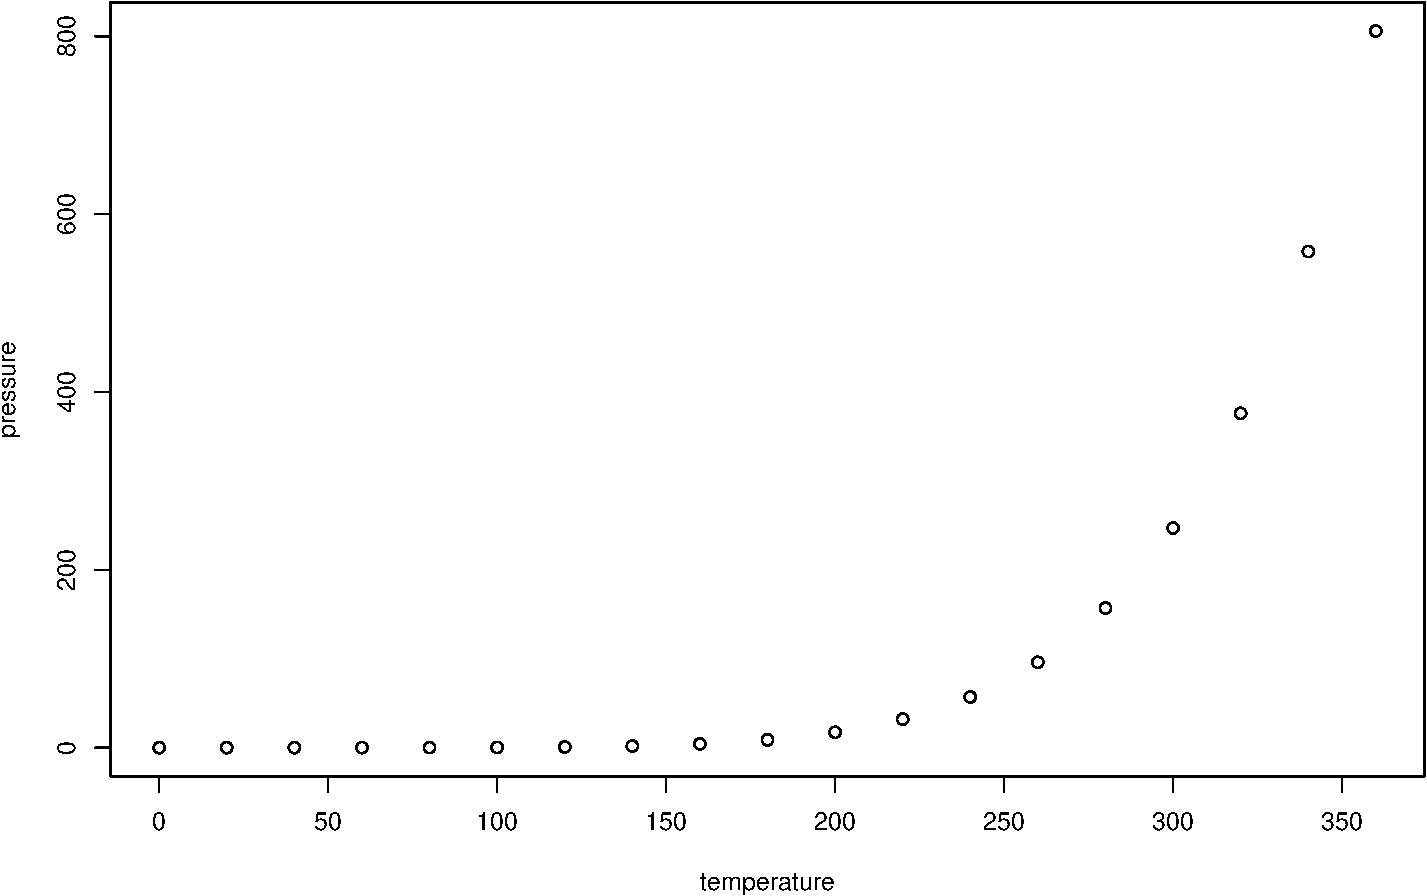
\includegraphics{slides_rmd_files/figure-beamer/pressure-1.pdf}

\end{frame}

\hypertarget{conclusion}{%
\section{Conclusion}\label{conclusion}}

\begin{frame}[fragile]{Conclusion}
\protect\hypertarget{conclusion-1}{}

To use this theme, download the \texttt{ubd\_beamer\_rmd.tex} file,
\texttt{.sty} files, and image files (for the logo and banner) from
\url{https://github.com/haziqj/ubd-beamer}, and place the files together
with your \texttt{.Rmd} source file. Use the sample
\texttt{slides\_rmd.Rmd} as a guide.

\end{frame}

\begin{frame}{End}
\protect\hypertarget{end}{}

\centering

\Huge Thank you!

\end{frame}

\begin{frame}{References}
\protect\hypertarget{references}{}

\hypertarget{refs}{}
\leavevmode\hypertarget{ref-casella2002statistical}{}%
Casella, George, and Roger L. Berger. 2002. \emph{Statistical
Inference}. 2nd ed. Pacific Grove, CA: Duxbury.

\leavevmode\hypertarget{ref-pawitan2001all}{}%
Pawitan, Yudi. 2001. \emph{In All Likelihood. Statistical Modelling and
Inference Using Likelihood}. Oxford University Press.

\leavevmode\hypertarget{ref-wasserman2013all}{}%
Wasserman, Larry. 2004. \emph{All of Statistics: A Concise Course in
Statistical Inference}. New York: Springer-Verlag.
\url{https://doi.org/10.1007/978-0-387-21736-9}.

\end{frame}


% % \begin{frame}[t,allowframebreaks,noframenumbering,plain]{References}
% 	\printbibliography[heading=none]
% \end{frame}
% 

\end{document}